% Large-Scale Mapping in Drupal with the Geocluster-Leaflet Stack
% Author:       Eric Paul
% Organization: Phase2
%
% This text and presentation is released and licensed under GPL 3.0.
% You are free to reuse and distribute as you wish.
% @see http://opensource.org/licenses/GPL-3.0

\documentclass{beamer}

\usetheme{Warsaw}
\usepackage{color}
\usepackage{graphicx}
\usepackage{textpos}

\definecolor{p2orange}{RGB}{253,121,0}
\definecolor{p2dark}{RGB}{40,47,54}
\setbeamercolor{palette primary}{use=structure,fg=white,bg=p2orange}
\setbeamercolor{palette quaternary}{use=structure,fg=white,bg=p2dark}
\setbeamercolor{normal text}{use=structure,fg=p2dark}
\setbeamercolor{item}{fg=p2orange}

% For the lower-right corner logo.
\logo{
\includegraphics[scale=0.2]{assets/p2-logo-pinwheel.png}}

\begin{document}

% Meta for title slide.
\title[Large-Scale Mapping in Drupal with Geocluster \& Leaflet]{Scalable, Server-side Mapping in Drupal with the Geocluster-Leaflet Stack}  
\author[@mpgeek]{Eric Paul (@mpgeek)\\ \vspace{0.5em}
\includegraphics[scale=0.25]{assets/p2-logo_small.jpg}}
\institute {Phase2 Technology}
\date{\today} 

\begin{frame} 
  \maketitle
\end{frame}

\frame{\frametitle{Table of contents}\tableofcontents} 

\section{Background} 

\frame{\frametitle{Mapping: What Is Going On Here?}
  \centerline{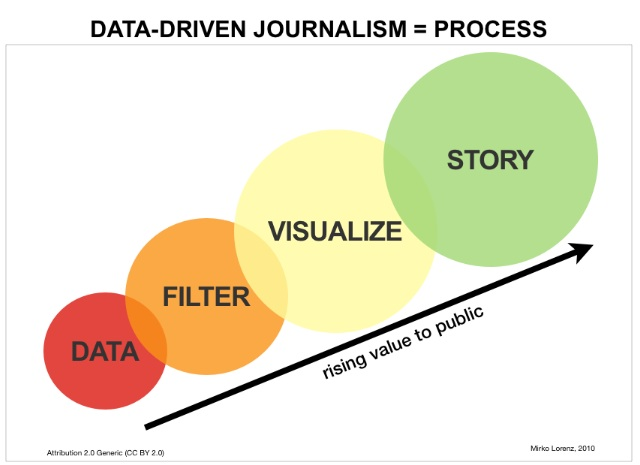
\includegraphics[scale=0.4]{assets/data-driven-journalism.jpg}}
}

\frame{\frametitle{The Process}
  \textbf{Data Driven Journalism as a \alert{Process}}
  \vspace{0.5em}
  \begin{itemize}
	\item Given a set of data
	\item And a question to be asked
	\item Find a useful visualization
	\item Data can then \alert{tell the story}
  \end{itemize}
  \pause
  \vspace{1em}
  This allows content authors to \alert{present data in context} in ways that would be \textcolor{p2orange}{difficult with words alone}.
  \vspace{0.5em}
  \begin{itemize}
    \item We can adopt this media-industry notion and generalize it to \alert{usability}.
  \end{itemize}
}

\frame{\frametitle{Mapping: Why is This Important?}
  \centerline{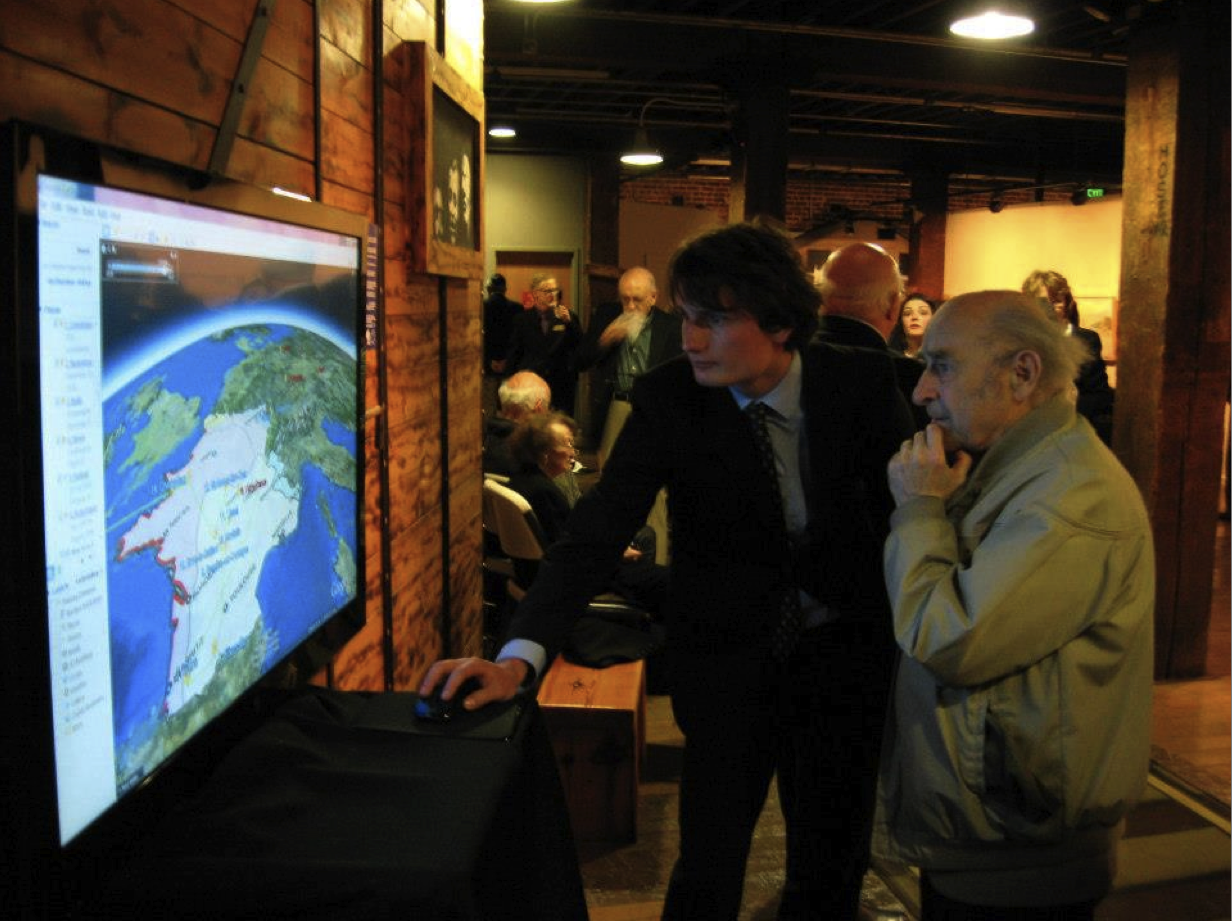
\includegraphics[scale=0.22]{assets/data-driven-journalism--example.png}}
}

\frame{\frametitle{The Problem: Dense-Point Data}
  \centerline{First pass: we have \alert{point crowding}.}
  \centerline{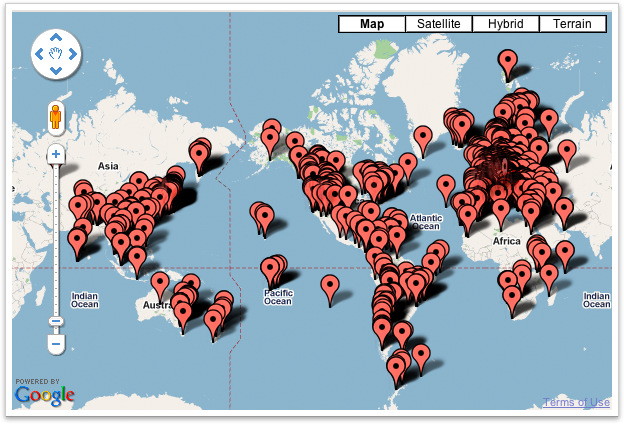
\includegraphics[scale=0.4]{assets/google-example_no-cluster.png}}
  \centerline{Really \alert{not usable}.}
}

\frame{\frametitle{One Solution: Client-Side Clustering}
  \centerline{First step: lets cluster on the \alert{client side}.}
  \centerline{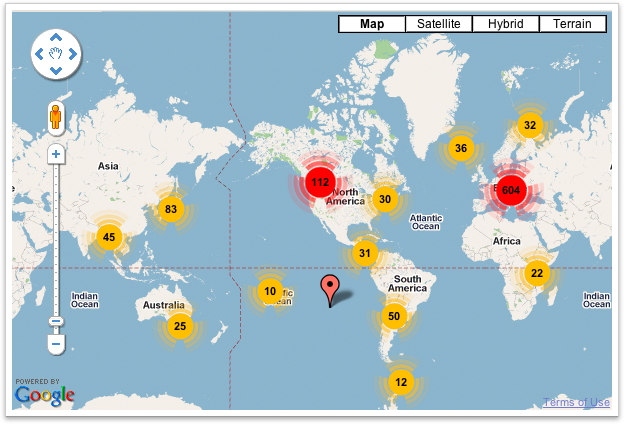
\includegraphics[scale=0.4]{assets/google-example_clustered.png}}
  \centerline{More usable, we gain context and can zoom in on areas of interest.}
}

\frame{\frametitle{Solution Breakdown: Clustering Thousands of Points}
  \centerline{What if we have \alert{thousands} of points?}
  \centerline{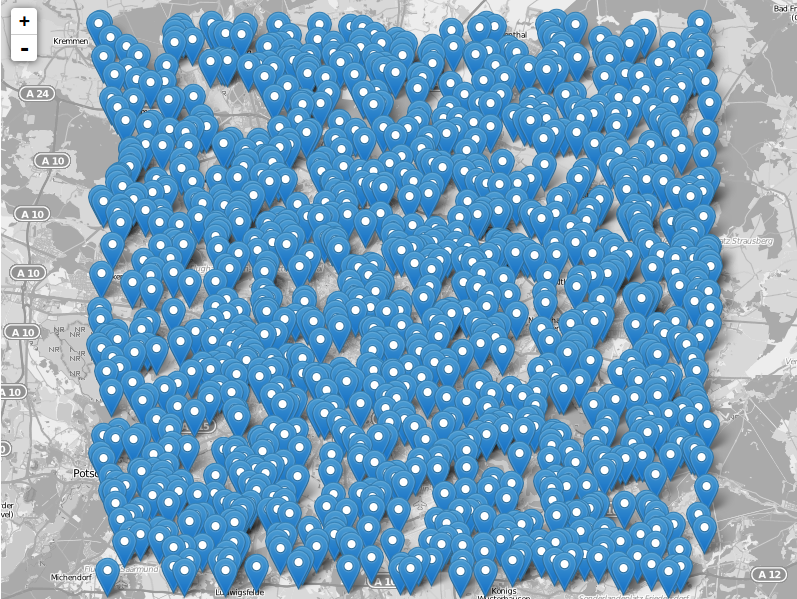
\includegraphics[scale=0.25]{assets/thousands-unclustered.png}}
  \centerline{Client-side clustering \alert{breaks down} upwards of a few hundred points.}
}

\frame{\frametitle{Roadblock: Client-Side Clustering at Large Scale}
  \textbf{Why Does it Break?}
  \vspace{0.5em}
  \begin{enumerate}
    \item Views (\textcolor{p2orange}{PHP}) renders each data point as a row of output, one at a time (thousands).
    \item Views (\textcolor{p2orange}{PHP}) renders the popup info (hidden) at page-load time.
    \item The mapping library (\textcolor{blue}{JS}) must parse the data.
    \item The mapping library (\textcolor{blue}{JS}) clusters the points.
    \item The mapping library (\textcolor{blue}{JS}) renders the map.
  \end{enumerate}
  \pause
  \vspace{1em}
  Both \textcolor{p2orange}{PHP} and \textcolor{blue}{JS} are asked to do too much at once.
  \begin{itemize}
    \item The \alert{breaking point} is about 300 data points (empirical).
  \end{itemize}
}

\frame{\frametitle{Client-Side Clustering Visualized}
  \centerline{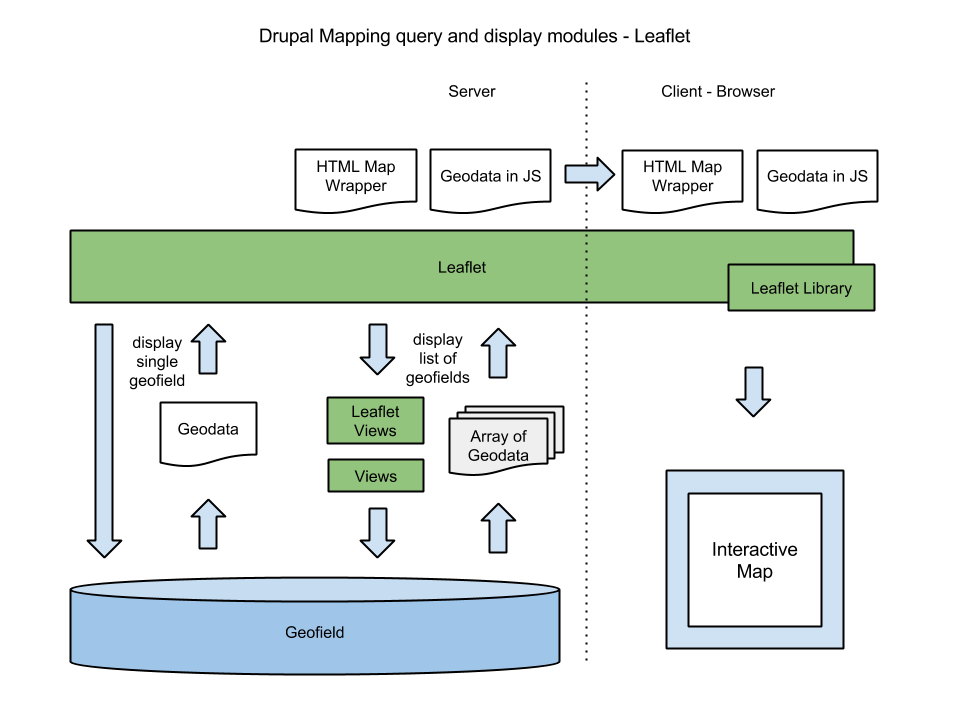
\includegraphics[scale=0.3]{assets/client-side-clustering.png}}
}

\frame{\frametitle{Demo}
  \centerline{\href{http://vistacampus.gov/map}{http://vistacampus.gov/map}}
  \centerline{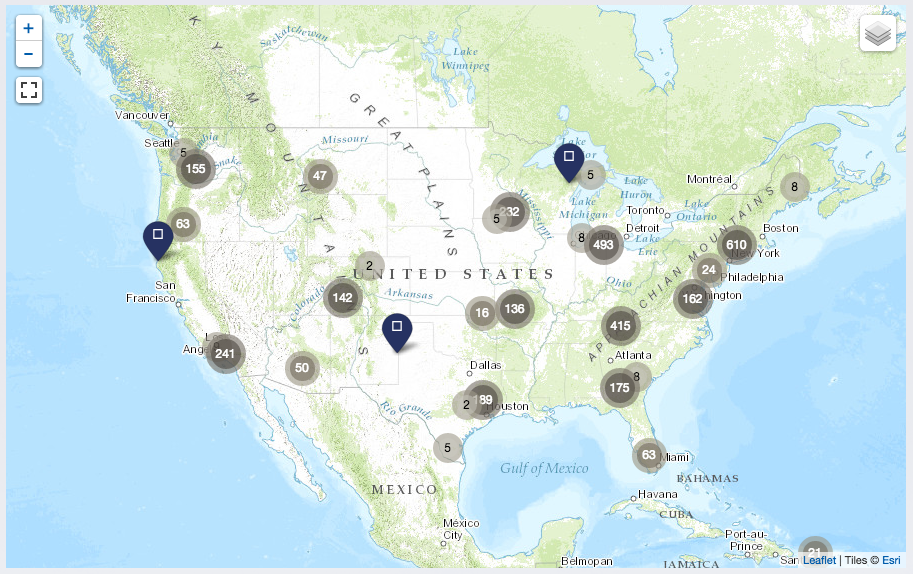
\includegraphics[scale=0.3]{assets/vista-map--static.png}}
}

\frame{\frametitle{Demo: Things of Note}
  \begin{itemize}
    \item Bounded mapping (bbox strategy)
    \item Load time under 1sec
    \item Clusters are single things, not collections of things
    \item On-demand, ajax-delivered infobubbles
    \item Dynamic reclustering on pan/zoom
    \item About 4K points 
    \item Layer interference (boo!)
  \end{itemize}
}

\frame{\frametitle{Starter Build}
  \textbf{If you really want to build this...}
  \begin{enumerate}
  	\item Clone the starter build
	\item Modify to suit
  \end{enumerate}
  \vspace{1em}
  \pause
  \textbf{Starter Build:}\\
  \href{http://cgit.drupalcode.org/geocluster/tree/modules/geocluster\_demo}{http://cgit.drupalcode.org/geocluster/tree/modules/geocluster\_demo}
  \begin{itemize}
    \item Instructions: \href{https://www.drupal.org/node/1962198}{https://www.drupal.org/node/1962198}
  \end{itemize}
  \vspace{1em}
  \pause
  \textbf{Why?}
  \begin{itemize}
    \item The configuration is tedious and complex.
    \item Way too easy to break to start from scratch.
  \end{itemize}
}

\section{The Geocluster-Leaflet Stack}

\frame{\frametitle{The Recipe}
  \textbf{Basic Recipe}
  \begin{itemize}
    \item Address Field (location storage)
    \item Geocoder (geocoding addresses, requires GeoPHP)
    \item Geofield (geocode storage)
    \item \textbf{Geocluster} (server-side clustering)
    \item Views
    \item Views GeoJSON (GeoJSON feeds)
    \item Leaflet GeoJSON (2.x for Panels support, 1.x for Bean)
    \item Leaflet Integration (requires Leaflet core library)
  \end{itemize}
  \vspace{1em}
  \pause
  But... we need lots of \alert{patches}.
}

\frame{\frametitle{A Working Model}
  The client build has been released as GPL2.0
  \begin{itemize}
    \item \href{https://github.com/mpgeek/Vista-Map}{https://github.com/mpgeek/Vista\-Map}
  \end{itemize}
  \vspace{1em}
  Patch mania! How about a \textcolor{p2orange}{makefile}?
  \begin{itemize}
    \item \href{https://github.com/mpgeek/Vista-Map/blob/master/vista\_map.make}{https://github.com/mpgeek/Vista-Map/blob/master/vista\_map.make}
  \end{itemize}
}

\frame{\frametitle{Client-Side Clustering Visualized (Redux)}
  \centerline{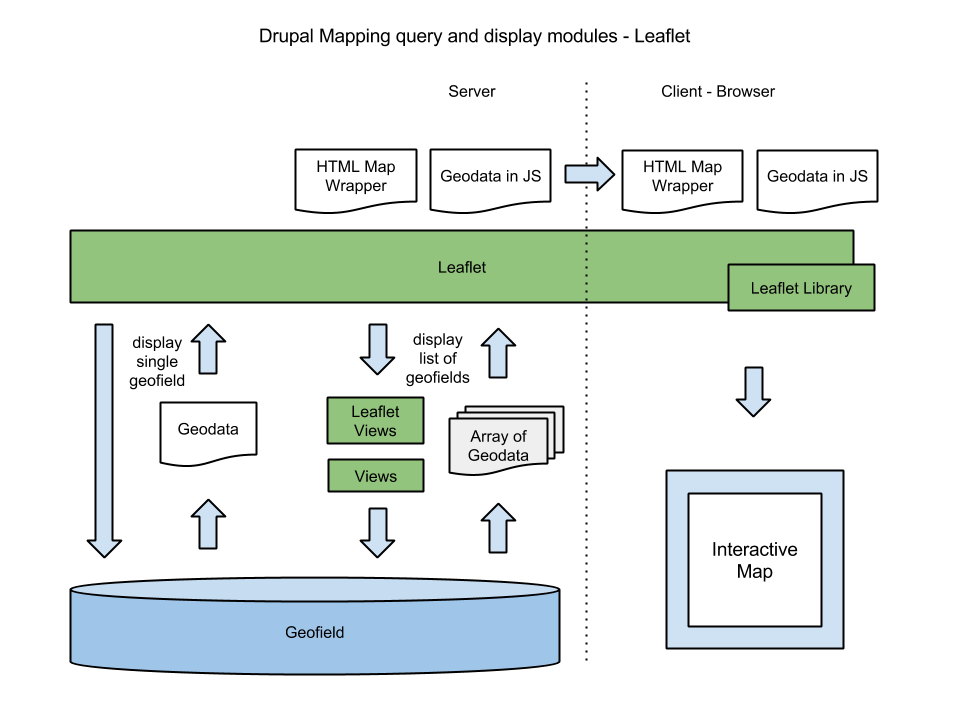
\includegraphics[scale=0.3]{assets/client-side-clustering.png}}
}

\frame{\frametitle{Server-Side Clustering with Geocluster Visualized}
  \centerline{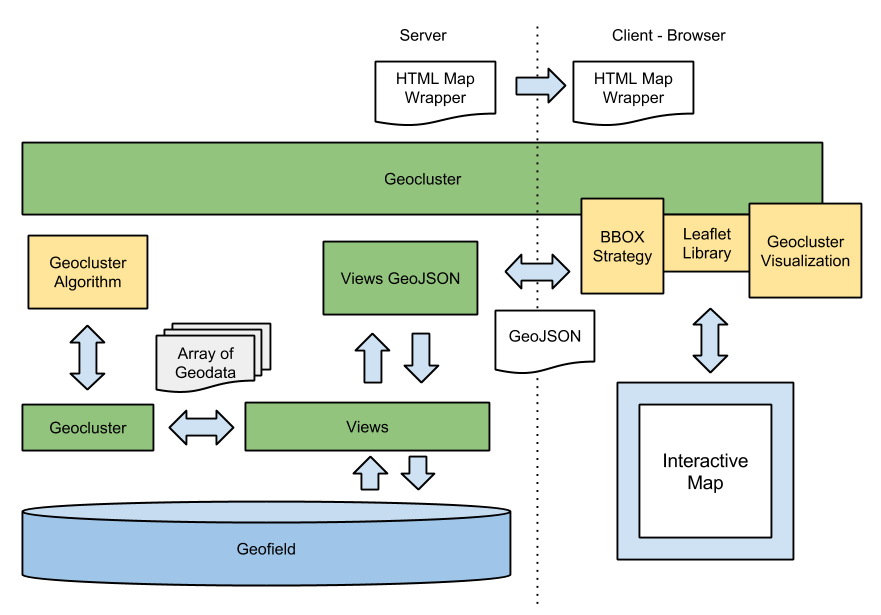
\includegraphics[scale=0.3]{assets/server-side-clustering--geocluster.png}}
}

\frame{\frametitle{Key Architectural Feature}
  \textbf{Geocluster Keys}
  \begin{itemize}
    \item Clustering is performed at the \alert{query level} by Geocluster
    \item \textcolor{p2orange}{PHP} and \textcolor{blue}{JS} only see the clusters as single (Views) rows.
    \item This feature alone is almost \alert{entirely responsible} for the performance gain.
  \end{itemize}
  \pause
  \vspace{1em}
  But How?
  \pause
  \begin{itemize}
    \item By \textcolor{p2orange}{geohashing}!
  \end{itemize}
}

\frame{\frametitle{Geocluster \& Geohash}
  \textbf{In a nutshell:}
  \begin{itemize}
    \item Geocluster adds a hierarchical, spatial index to geofields based on the Geohash algorithm.
    \item Each geofield has columns for varying levels of precision (geohash index) created/updated on \textcolor{gray}{\texttt{entity\_save}}.
    \item A query for points/clusters specifies a geohash index and asks for clusters based on that index.
  \end{itemize}
  \pause
  \vspace{1em}
  \textbf{Notice:}
  \begin{itemize}
    \item The clustering information is created when the content is \alert{created}.
    \item A request for points and clusters \alert{doesn't actually cluster}. Rather it's a \alert{simple query} of a spatial index. 
  \end{itemize}
}

\section{Customization Towards an Application}

\frame{\frametitle{Near-point Clusters vs. Exact-point Clusters}
  \textbf{Monolithic Clusters}
  \vspace{2em}
  \begin{itemize}
    \item Leaflet doesn't discern between points that are \textcolor{p2orange}{near to one another} versus multiple points at the \alert{same location}.
    \vspace{1.5em}
    \item We needed to create two cluster types, on for each condition.
    \vspace{1.5em}
    \pause
    \item \href{https://github.com/mpgeek/Vista-Map/blob/master/vista\_map.module\#L115}{\texttt{\textcolor{gray}{vista\_map.module}}, lines 115-155}
  \end{itemize}
}

\frame{\frametitle{On-Demand Popups}
  \textbf{AJAX!}
  \vspace{1.5em}
  \begin{itemize}
    \item We don't load the popup info into the DOM at map-load time (performance tactic).
    \vspace{1em}
    \item We needed to load them on demand and allow them to be cached.
    \vspace{1em}
    \pause
    \item \href{https://github.com/mpgeek/Vista-Map/blob/master/vista\_map.js\#L123}{\texttt{\textcolor{gray}{vista\_map.js}}, lines 324-404}
  \end{itemize}
}

\frame{\frametitle{Current-user Zoom}
  \textbf{Focus the Map on the Current-user's Location}
  \vspace{1.5em}
  \begin{itemize}
    \item One of the purposes of the map was to emphasize making local connections.
    \vspace{1em}
    \item We wanted to zoom in on the currently logged-in user.
    \vspace{1em}
    \pause
    \item \href{https://github.com/mpgeek/Vista-Map/blob/master/vista\_map.module\#L290}{\texttt{\textcolor{gray}{vista\_map.module}}, lines 290-351}
  \end{itemize}
}

\frame{\frametitle{Limit Geocoder Granularity}
  \textbf{Geocode to Center of ZIP-code Only}
  \vspace{1.5em}
  \begin{itemize}
    \item One of two data layers needed to geocode only to ZIP-code precision.
    \vspace{1em}
    \item Removing more-specific information and passing abbreviated info only to geocoder.
    \vspace{1em}
    \pause
    \item \href{https://github.com/mpgeek/Vista-Map/blob/master/vista\_map.module\#L12}{\texttt{\textcolor{gray}{vista\_map.module}}, lines 12-72}
  \end{itemize}
}

\frame{\frametitle{Multiple Data Layers}
  \textbf{Implement Data Layering and Panels Support}
  \vspace{1.5em}
  \begin{itemize}
    \item OG membership drove layer membership, and source geofield.
   \vspace{1em}
    \item Views necessitated that different source geofields be separate data layers.
    \vspace{1em}
    \pause
    \item Contiributed the 2.x branch of Leaflet GeoJSON for panels support with multiple data layers (\href{https://www.drupal.org/node/2225815}{https://www.drupal.org/node/2225815})
  \end{itemize}
}

\frame{\frametitle{Scalability Requirement}
  \textbf{How big did we need to go?}
  \vspace{0.5em}
  \begin{itemize}
    \item Mapping user profiles, about 18k users were migrated
    \vspace{0.5em}
    \item Originally, it was expected that all users would be map
    \vspace{0.5em}
    \item Application scale, then is $10\textsuperscript{4}$
  \end{itemize}
  \vspace{1em}
  \pause
  Geocluster's clustering backend is \alert{pluggable}
  \vspace{1em}
  \begin{itemize}
  	\item PHP clustering (post-query clusternig)
	\vspace{0.5em}
	\item MySQL clustering (query-level clustering)
	\vspace{0.5em}
	\item Apache solr clustering (alternative query-level clustering)
  \end{itemize}
}

\frame{\frametitle{Scalability Metrics}
  \centerline{\textcolor{p2orange}{Cold caches}}
  \centerline{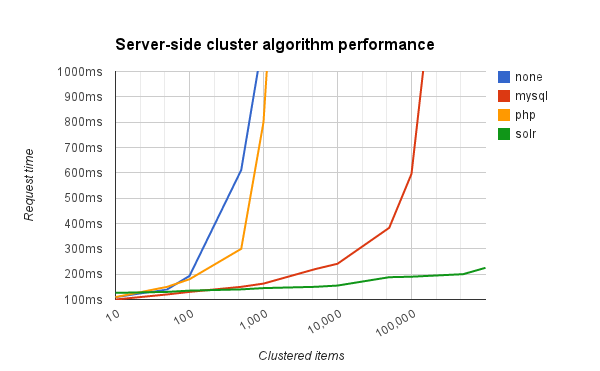
\includegraphics[scale=0.45]{assets/geocluster-performance.png}}
  \centerline{We implemented \alert{MySQL} clustering}
}

\frame{\frametitle{Possible Improvements}
  \textbf{Geocluster}
  \begin{itemize}
    \item Progressively enhance with client side clustering below a certain point threshold. \href{https://www.drupal.org/node/1914704}{https://www.drupal.org/node/1914704}
    \pause
    \vspace{0.5em}
    
  \end{itemize}
}

\frame{\frametitle{Possible Improvements}
  \textbf{Leaflet GeoJSON}
  \begin{itemize}
    \item Collapse clusters to a single layer to eliminate layer interference.
    \vspace{0.5em}
    \pause
    \item Make data feeds cacheable by quantizing bounding box parameters.\\ \textcolor{gray}{\footnotesize{\texttt{/\$view\_url?bbox=\$left,\$right,\$top,\$bottom?zoom=\$zoom\_level}}}
    \vspace{0.5em}
    \begin{itemize}
      \item The \texttt{\textcolor{gray}{bbox}} arguments are floating-point numbers that depend on viewport size and zoom. \alert{Takes a long time for caches to warm up for non-mobile viewports}.
      \vspace{0.5em}
      \item \href{https://www.drupal.org/node/1868982}{https://www.drupal.org/node/1868982}
    \end{itemize}
  \end{itemize}
}

\section{Takeaways}

\frame{\frametitle{Take-out Knowledge}
  \textbf{What we know}
  \vspace{1em}
  \begin{itemize}
    \item Large-scale mapping is now possible in Drupal.
    \vspace{0.5em}
    \item Geocluster needs work.
    \vspace{0.5em}
    \item Leaflet GeoJSON needs work.
    \vspace{0.5em}
    \item Despite that, production-quality map applications can now be built.
    \vspace{0.5em}
    \pause
    \item \alert{You will need a debugger}.
  \end{itemize}
}

\frame{\frametitle{References \& Resources}
  \textbf{Things we saw and more resources:}
  \begin{itemize}
  	\item Map application in production: \href{http://www.vistacampus.gov/map}{http://www.vistacampus.gov/map}
	\vspace{1em}
	\item Map application Drupal feature: \href{https://github.com/mpgeek/Vista-Map}{https://github.com/mpgeek/Vista-Map}
    \vspace{1em}
    \item Geohash Algorithm:\\ \href{http://en.wikipedia.org/wiki/Geohash}{http://en.wikipedia.org/wiki/Geohash}
    \vspace{1em}
    \item Geocluster Master's Thesis (by @dasjo): \href{http://dasjo.at/thesis}{http://dasjo.at/thesis}
  \end{itemize}
}

\frame{\frametitle{Questions?}
  \centerline{
\includegraphics[scale=0.6]{assets/questions.jpg}}
  \vspace{1em}
  \centerline{Find me on twitter, IRC, or drupal.org: @mpgeek}
}

%%\frame{\frametitle{Title} 
Each frame should have a title.
}
%\subsection{Subsection no.1.1  }
\frame{ 
Without title somethink is missing. 
}


%\section{Section no. 2} 
%\subsection{Lists I}
\frame{\frametitle{unnumbered lists}
\begin{itemize}
\item Introduction to  \LaTeX  
\item Course 2 
\item Termpapers and presentations with \LaTeX 
\item Beamer class
\end{itemize} 
}

\frame{\frametitle{lists with pause}
\begin{itemize}
\item Introduction to  \LaTeX \pause 
\item Course 2 \pause 
\item Termpapers and presentations with \LaTeX \pause 
\item Beamer class
\end{itemize} 
}

%\subsection{Lists II}
\frame{\frametitle{numbered lists}
\begin{enumerate}
\item Introduction to  \LaTeX  
\item Course 2 
\item Termpapers and presentations with \LaTeX 
\item Beamer class
\end{enumerate}
}
\frame{\frametitle{numbered lists with pause}
\begin{enumerate}
\item Introduction to  \LaTeX \pause 
\item Course 2 \pause 
\item Termpapers and presentations with \LaTeX \pause 
\item Beamer class
\end{enumerate}
}

%\section{Section no.3} 
%\subsection{Tables}
\frame{\frametitle{Tables}
\begin{tabular}{|c|c|c|}
\hline
\textbf{Date} & \textbf{Instructor} & \textbf{Title} \\
\hline
WS 04/05 & Sascha Frank & First steps with  \LaTeX  \\
\hline
SS 05 & Sascha Frank & \LaTeX \ Course serial \\
\hline
\end{tabular}}


\frame{\frametitle{Tables with pause}
\begin{tabular}{c c c}
A & B & C \\ 
\pause 
1 & 2 & 3 \\  
\pause 
A & B & C \\ 
\end{tabular} }


%\section{Section no. 4}
%\subsection{blocs}
\frame{\frametitle{blocs}

\begin{block}{title of the bloc}
bloc text
\end{block}

\begin{exampleblock}{title of the bloc}
bloc text
\end{exampleblock}


\begin{alertblock}{title of the bloc}
bloc text
\end{alertblock}
}

%\section{Section no. 5}
%\subsection{split screen}

\frame{\frametitle{splitting screen}
\begin{columns}
\begin{column}{5cm}
\begin{itemize}
\item Beamer 
\item Beamer Class 
\item Beamer Class Latex 
\end{itemize}
\end{column}
\begin{column}{5cm}
\begin{tabular}{|c|c|}
\hline
\textbf{Instructor} & \textbf{Title} \\
\hline
Sascha Frank &  \LaTeX \ Course 1 \\
\hline
Sascha Frank &  Course serial  \\
\hline
\end{tabular}
\end{column}
\end{columns}
}

%\subsection{Pictures} 
\frame{\frametitle{pictures in latex beamer class}
\begin{figure}
%\includegraphics[scale=0.5]{PIC1} 
\caption{show an example picture}
\end{figure}}

%\subsection{joining picture and lists} 

\frame{
\frametitle{pictures and lists in beamer class}
\begin{columns}
\begin{column}{5cm}
\begin{itemize}
\item<1-> subject 1
\item<3-> subject 2
\item<5-> subject 3
\end{itemize}
\vspace{3cm} 
\end{column}
\begin{column}{5cm}
\begin{overprint}
%\includegraphics<2>{PIC1}
%\includegraphics<4>{PIC2}
%\includegraphics<6>{PIC3}
\end{overprint}
\end{column}
\end{columns}}

\end{document}